
% Maybe some stuff about template metaprogramming in this chapter?

\chapter{User documentation}

\section{Target audience}

This document expects the reader to have a basic understanding of template
metaprogramming in C++.

%TODO

\section{Main concepts}

%TODO

\section{Installation}

Metashell supports the following platforms:
\begin{itemize}
    \item Linux
    \item FreeBSD
    \item OpenBSD
    \item OS X
    \item Windows
\end{itemize}

In this section, installation instructions only for Linux is described.
Instructions for other platforms can be found in the README.md file shipped
with Metashell.

\subsection{Dependencies}

Install the dependent libraries and tools:

\begin{itemize}
    \item Termcap and Readline (version 6.3 or newer)
    \item CMake (2.18.12.2 or newer)
\end{itemize}

Acquire the source code from Github\cite{github} or any release site, and cd
into the source directory:

\begin{itemize}
    \item \verb$cd metashell$
\end{itemize}

Build Clang with Templight\cite{templight}:

\begin{itemize}
    \item \verb$cd templight$
    \item \verb$mkdir build$
    \item \verb$cd build$
    \item \verb$cmake ../llvm -DLIBCLANG_BUILD_STATIC=ON$
    \item \verb$make clang$
    \item \verb$make libclang$
    \item \verb$make libclang_static$
    \item \verb$cd ..$
\end{itemize}

\subsection{Building}

Now compile Metashell:

\begin{itemize}
    \item \verb$mkdir bin$
    \item \verb$cd bin$
    \item \verb$cmake ..$
    \item \verb$make$
\end{itemize}

%TODO what kind of files appeared?

\subsection{Running tests}

To make sure everything will work correctly, running tests is advised:

\begin{itemize}
    \item \verb$test/metashell_test$
\end{itemize}

\section{Basic Usage}

Start metashell by running \verb$app/metashell$.

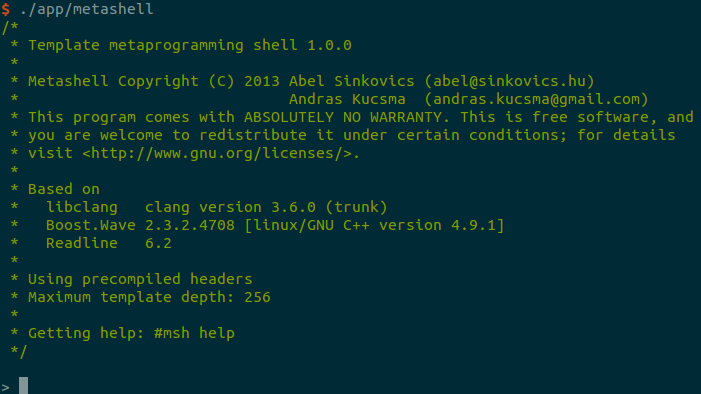
\includegraphics[width=1\textwidth]{img/splash.eps}

%TODO maybe mention, that "> " is metashell?
After a splash screen is shown, an interactive shell with \verb$"> "$
prompt string appears. This is the place, where the C++ code environment
required by the metaprogram can be entered.


%TODO moar usage

\section{Command reference}

In the following section, the following notations are used: command parameters
that are in square brackets are optional. Parameters that are between angle
brackets have to be replaced by the user with something.

\subsection{evaluate}

Usage: \verb$evaluate [-full] [<type>]$

Evaluate and start debugging a new metaprogram.

Evaluating a metaprogram using the \verb$-full$ qualifier will expand all
Memoization events.

If called without <type>, then the last evaluated metaprogram will be
reevaluated.

Previous breakpoints are cleared.

Unlike metashell, evaluate doesn't use metashell::format to avoid cluttering
the debugged metaprogram with unrelated code. If you need formatting, you can
explicitly enter \verb$metashell::format< <type> >::type$ for the same effect.

\subsection{step}

Usage: \verb$step [over] [n]$

Step the program.

Argument n means step n times. n defaults to 1 if not specified.
Negative n means step the program backwards.

Use of the \verb$over$ qualifier will jump over sub instantiations.

\subsection{rbreak}

Usage: \verb$rbreak <regex>$

Add breakpoint for all types matching \verb$<regex>$.



\subsection{continue}

Usage: \verb$continue [n]$

Continue program being debugged.

The program is continued until the nth breakpoint or the end of the program
is reached. n defaults to 1 if not specified.
Negative n means continue the program backwards.

\subsection{forwardtrace}

Usage: \verb$forwardtrace|ft [n]$

Print forwardtrace from the current point.

The n specifier limits the depth of the trace. If n is not specified, then the
trace depth is unlimited.

\subsection{backtrace}

Usage: \verb$backtrace|bt $

Print backtrace from the current point.



\subsection{help}

Usage: \verb$help [<command>]$

Show help for commands.

If <command> is not specified, show a list of all available commands.

\subsection{quit}

Usage: \verb$quit $

Quit metadebugger.





